
\chapter{Đặc tả các use-case}

Hệ thống "Chương trình hỗ trợ dạy và học Vật lý lớp 11" bao gồm các tác nhân (actors) chính: Người dùng (học sinh, giáo viên) và Quản trị viên (Admin). Hệ thống được chia thành bốn phân vùng chức năng chính: (1) Xác thực và Phân quyền, (2) Sách giáo khoa điện tử và Mô phỏng 3D, (3) Đề luyện tập, và (4) Quản trị hệ thống.

\section{Sơ đồ Use-case tổng quát}

\begin{figure}[H]
    \centering
    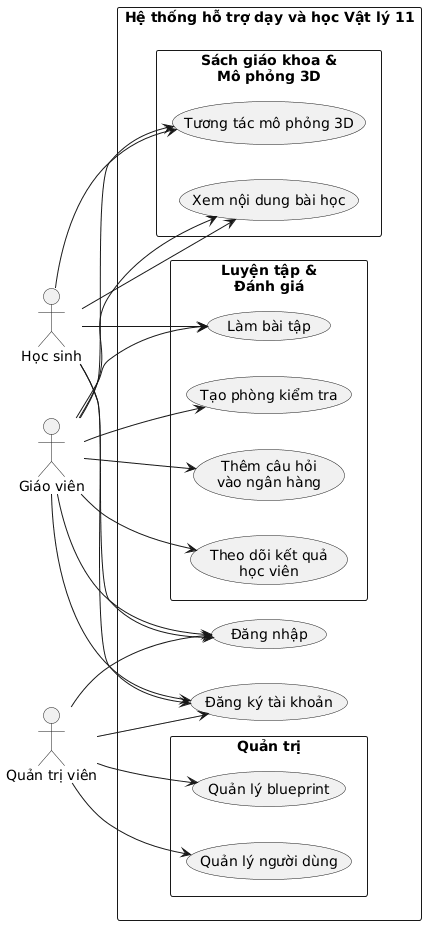
\includegraphics[width=\textwidth,
    height=0.8\textheight,
    keepaspectratio]{Images/Phan_tich_Thiet_ke_he_thon/Usecase Physics Book.png}
    \vspace{0.5cm}
    \caption{Sơ đồ Use-case tổng quát của hệ thống}
    \label{fig:usecase-overall}
\end{figure}

\section{Đặc tả chi tiết các Use-case}

\subsection{Phân vùng Xác thực và Phân quyền}

\begin{longtable}{|p{0.18\textwidth}|p{0.75\textwidth}|}
\hline
\textbf{Tên Usecase} & \textbf{Đăng ký tài khoản} \\
\hline
\textbf{Actors} & Người dùng (Học sinh) \\
\hline
\textbf{Mô tả} & Cho phép người dùng tạo tài khoản mới để truy cập các chức năng của hệ thống: xem bài học, tương tác với mô phỏng 3D, làm bài tập, và theo dõi tiến độ học tập. \\
\hline
\textbf{Trigger} & Người dùng nhấn nút "Đăng ký" tại Trang chủ hệ thống. \\
\hline
\textbf{Tiền điều kiện} & Dịch vụ xác thực và cơ sở dữ liệu sẵn sàng. \\
\hline
\textbf{Hậu điều kiện} & Tài khoản mới được lưu vào cơ sở dữ liệu với vai trò mặc định là \texttt{user}. \\
\hline
\textbf{Luồng chính} &
\vspace{-\baselineskip}
\begin{enumerate}[topsep=2pt, itemsep=0pt]
    \item Hệ thống hiển thị form Đăng ký với các trường: Họ tên, Email, Tên đăng nhập, Mật khẩu, Xác nhận mật khẩu.
    \item Người dùng nhập đầy đủ thông tin vào các trường.
    \item Người dùng nhấn nút "Đăng ký".
    \item Hệ thống kiểm tra tính hợp lệ của dữ liệu:
    \begin{itemize}[topsep=0pt, itemsep=0pt]
        \item Tên đăng nhập chưa tồn tại trong hệ thống.
        \item Email đúng định dạng và chưa được sử dụng.
        \item Mật khẩu có độ dài $\geq$ 8 ký tự, bao gồm chữ hoa, chữ thường và số.
        \item Mật khẩu và Xác nhận mật khẩu trùng khớp.
    \end{itemize}
    \item Hệ thống mã hóa mật khẩu bằng \texttt{bcryptjs} (salt rounds = 10).
    \item Hệ thống lưu thông tin tài khoản vào collection \texttt{users} trong MongoDB.
    \item Hệ thống hiển thị thông báo "Đăng ký thành công" và chuyển hướng đến trang Đăng nhập.
    \item Kết thúc Use-case.
\end{enumerate} \\
\hline
\textbf{Luồng thay thế} &
\vspace{-\baselineskip}
\begin{enumerate}[topsep=2pt, itemsep=0pt]
    \item[2a.] Người dùng bỏ trống một hoặc nhiều trường bắt buộc:
    \begin{itemize}[topsep=0pt, itemsep=0pt]
        \item Hệ thống hiển thị thông báo lỗi màu đỏ bên dưới trường bị bỏ trống: "Vui lòng nhập trường này".
        \item Người dùng quay lại bước 2.
    \end{itemize}
    \item[4a.] Tên đăng nhập đã tồn tại:
    \begin{itemize}[topsep=0pt, itemsep=0pt]
        \item Hệ thống hiển thị thông báo: "Tên đăng nhập đã được sử dụng. Vui lòng chọn tên khác."
        \item Người dùng quay lại bước 2.
    \end{itemize}
    \item[4b.] Email không đúng định dạng:
    \begin{itemize}[topsep=0pt, itemsep=0pt]
        \item Hệ thống hiển thị thông báo: "Email không đúng định dạng."
        \item Người dùng quay lại bước 2.
    \end{itemize}
    \item[4c.] Mật khẩu và Xác nhận mật khẩu không khớp:
    \begin{itemize}[topsep=0pt, itemsep=0pt]
        \item Hệ thống hiển thị thông báo: "Xác nhận mật khẩu không trùng khớp."
        \item Người dùng quay lại bước 2.
    \end{itemize}
\end{enumerate} \\
\hline
\textbf{Ngoại lệ} &
\vspace{-\baselineskip}
\begin{enumerate}[topsep=2pt, itemsep=0pt]
    \item[5a.] Không thể kết nối đến máy chủ xác thực hoặc cơ sở dữ liệu:
    \begin{itemize}[topsep=0pt, itemsep=0pt]
        \item Hệ thống hiển thị thông báo: "Lỗi kết nối máy chủ. Vui lòng thử lại sau."
        \item Kết thúc Use-case.
    \end{itemize}
\end{enumerate} \\
\hline
\caption{Đặc tả chi tiết Use-case Đăng ký tài khoản}
\label{table:uc-register}
\end{longtable}

\clearpage

\begin{longtable}{|p{0.18\textwidth}|p{0.75\textwidth}|}
\hline
\textbf{Tên Usecase} & \textbf{Đăng nhập} \\
\hline
\textbf{Actors} & Người dùng (Học sinh), Giáo viên, Quản trị viên \\
\hline
\textbf{Mô tả} & Cho phép người dùng đăng nhập vào hệ thống để truy cập các chức năng tương ứng với vai trò được phân quyền. \\
\hline
\textbf{Trigger} & Actor nhấn nút "Đăng nhập" tại Trang chủ hệ thống. \\
\hline
\textbf{Tiền điều kiện} & 
\vspace{-\baselineskip}
\begin{itemize}[topsep=2pt, itemsep=0pt]
    \item Actor đã có tài khoản được tạo trong hệ thống.
    \item Dịch vụ xác thực sẵn sàng.
\end{itemize} \\
\hline
\textbf{Hậu điều kiện} & 
\vspace{-\baselineskip}
\begin{itemize}[topsep=2pt, itemsep=0pt]
    \item Actor đăng nhập thành công và được chuyển hướng đến trang chức năng tương ứng với vai trò.
    \item JWT token được tạo và lưu vào cookie/httpOnly storage.
\end{itemize} \\
\hline
\textbf{Luồng chính} &
\vspace{-\baselineskip}
\begin{enumerate}[topsep=2pt, itemsep=0pt]
    \item Hệ thống hiển thị form Đăng nhập với các trường: Tên đăng nhập, Mật khẩu.
    \item Actor nhập Tên đăng nhập và Mật khẩu.
    \item Actor nhấn nút "Đăng nhập".
    \item Hệ thống xác thực thông tin đăng nhập: kiểm tra tên đăng nhập tồn tại, so sánh mật khẩu đã băm với mật khẩu trong cơ sở dữ liệu.
    \item Hệ thống tạo JWT token (thời hạn 8 giờ) chứa thông tin: user ID, vai trò (\texttt{user}/\texttt{admin}).
    \item Hệ thống chuyển hướng Actor đến trang tương ứng:
    \begin{itemize}[topsep=0pt, itemsep=0pt]
        \item \texttt{user} → Trang chủ học tập (danh sách bài học và mô phỏng).
        \item \texttt{admin} → Trang Dashboard quản trị.
    \end{itemize}
    \item Kết thúc Use-case.
\end{enumerate} \\
\hline
\textbf{Luồng thay thế} &
\vspace{-\baselineskip}
\begin{enumerate}[topsep=2pt, itemsep=0pt]
    \item[2a.] Actor bỏ trống Tên đăng nhập hoặc Mật khẩu:
    \begin{itemize}[topsep=0pt, itemsep=0pt]
        \item Hệ thống hiển thị thông báo lỗi: "Vui lòng nhập đầy đủ thông tin."
        \item Actor quay lại bước 2.
    \end{itemize}
    \item[4a.] Thông tin đăng nhập không hợp lệ (sai tên đăng nhập hoặc mật khẩu):
    \begin{itemize}[topsep=0pt, itemsep=0pt]
        \item Hệ thống hiển thị thông báo: "Tên đăng nhập hoặc mật khẩu không đúng."
        \item Actor quay lại bước 2.
    \end{itemize}
\end{enumerate} \\
\hline
\textbf{Ngoại lệ} &
\vspace{-\baselineskip}
\begin{enumerate}[topsep=2pt, itemsep=0pt]
    \item[4b.] Không thể kết nối đến máy chủ xác thực:
    \begin{itemize}[topsep=0pt, itemsep=0pt]
        \item Hệ thống hiển thị thông báo: "Lỗi kết nối máy chủ. Vui lòng thử lại sau."
        \item Kết thúc Use-case.
    \end{itemize}
\end{enumerate} \\
\hline
\caption{Đặc tả chi tiết Use-case Đăng nhập}
\label{table:uc-login}
\end{longtable}

\clearpage

\subsection{Phân vùng Sách giáo khoa điện tử và Mô phỏng 3D}

\begin{longtable}{|p{0.18\textwidth}|p{0.75\textwidth}|}
\hline
\textbf{Tên Usecase} & \textbf{Xem nội dung bài học \& Tương tác với Mô phỏng 3D} \\
\hline
\textbf{Actors} & Người dùng (Học sinh), Giáo viên \\
\hline
\textbf{Mô tả} & 
Cho phép người dùng xem nội dung bài học dưới dạng slide trình chiếu, tương tác với các mô phỏng đã được tích hợp, điều chỉnh tham số vật lý, xem đồ thị phân tích thời gian thực. \\
\hline
\textbf{Trigger} & 
Người dùng truy cập vào phân vùng \textit{Sách giáo khoa điện tử} từ menu chính. \\
\hline
\textbf{Tiền điều kiện} & 
\vspace{-\baselineskip}
\begin{itemize}[topsep=2pt, itemsep=0pt]
    \item Người dùng đã đăng nhập vào hệ thống.
    \item Nội dung bài học và mô phỏng 3D đã được triển khai trong hệ thống.
\end{itemize} \\
\hline
\textbf{Hậu điều kiện} & 
\vspace{-\baselineskip}
\begin{itemize}[topsep=2pt, itemsep=0pt]
    \item Tiến độ xem bài học được ghi nhận vào hồ sơ người dùng.
    \item Các tham số mô phỏng được khôi phục về mặc định khi rời khỏi trang.
\end{itemize} \\
\hline
\textbf{Luồng chính} &
\vspace{-\baselineskip}
\begin{enumerate}[topsep=2pt, itemsep=0pt]
    \item Hệ thống hiển thị danh sách các bài học thuộc Chương 1 (Dao động) và Chương 2 (Sóng).
    \item Người dùng chọn một bài học để xem.
    \item Hệ thống hiển thị nội dung bài học dưới dạng slide trình chiếu, bao gồm:
    \begin{itemize}[topsep=0pt, itemsep=0pt]
        \item Văn bản lý thuyết được định dạng.
        \item Công thức toán học/vật lý hiển thị bằng KaTeX/LaTeX.
        \item Hình ảnh minh họa.
    \end{itemize}
    \item Người dùng điều hướng giữa các slide bằng chuột hoặc bàn phím (phím mũi tên).
    \item Tại slide cuối, hệ thống hiển thị mô phỏng 3D tương tác liên quan. Người dùng có thể chọn \textit{Tương tác với mô phỏng} (bước 5a) hoặc đi tiếp đến bước 6.
    \item Người dùng có thể chọn chức năng mở rộng: \textit{Làm bài tập mẫu} (bước 6).
    \item Hệ thống đánh dấu bài học đã hoàn thành nếu người dùng đã thực hiện các thao tác cần thiết.
    \item Kết thúc Use-case.
\end{enumerate} \\
\hline
\end{longtable}

\clearpage

% === PHẦN TIẾP THEO CỦA BẢNG DÀI (LUỒNG THAY THẾ & NGOẠI LỆ) ===

\begin{longtable}{|p{0.18\textwidth}|p{0.75\textwidth}|}
\hline
\textbf{Luồng thay thế} &
\vspace{-\baselineskip}
\begin{enumerate}[topsep=2pt, itemsep=0pt]
    \item[5a.] Người dùng chọn \textit{Tương tác với mô phỏng}:
    \begin{itemize}[topsep=0pt, itemsep=0pt]
        \item Hệ thống chuyển đến giao diện mô phỏng 3D tương ứng. Các mô phỏng có sẵn:
        \begin{enumerate}[label=\textbf{Sim \arabic*}, topsep=0pt, itemsep=0pt]
            \item \textbf{Con lắc đơn}: Kéo thả quả nặng, điều chỉnh $L$, $b$, xem đồ thị năng lượng.
            \item \textbf{Con lắc lò xo}: Kéo thả vật nặng, điều chỉnh $k$, $m$, $b$.
            \item \textbf{Sóng dọc \& Sóng ngang}: So sánh hai loại sóng, điều chỉnh $A$, $\lambda$, $f$.
            \item \textbf{Sóng trên dây}: Chọn chế độ liên tục/xung, điều kiện biên.
            \item \textbf{Giao thoa sóng}: 6.400 điểm giao thoa (InstancedMesh), vân hyperbol.
            \item \textbf{Sóng điện từ}: Quan sát $\vec{E} \perp \vec{B} \perp \vec{v}$.
            \item \textbf{Sonar}: Dò địa hình đáy biển 3D.
        \end{enumerate}
        \item Trong mỗi mô phỏng, người dùng có thể:
        \begin{itemize}[topsep=0pt, itemsep=0pt]
            \item Điều chỉnh tham số qua thanh trượt.
            \item Bật/tắt thành phần hiển thị qua checkbox.
            \item Điều khiển camera 3D (Xoay/Pan/Zoom).
            \item Xem đồ thị phân tích thời gian thực trong tab "Đồ Thị".
            \item Phát/Tạm dừng/Đặt lại mô phỏng.
            \item Chuyển đổi chế độ toàn màn hình.
        \end{itemize}
        \item Quay lại bước 6.
    \end{itemize}
    \item[6a.] Người dùng chọn \textit{Làm bài tập mẫu}:
    \begin{itemize}[topsep=0pt, itemsep=0pt]
        \item Hệ thống hiển thị bài tập mẫu kèm lời giải chi tiết dạng slide.
        \item Người dùng tự giải, sau đó đối chiếu với lời giải mẫu.
        \item Quay lại bước 7.
    \end{itemize}
\end{enumerate} \\
\hline
\textbf{Ngoại lệ} &
\vspace{-\baselineskip}
\begin{enumerate}[topsep=2pt, itemsep=0pt]
    \item[E1.] Trình duyệt không hỗ trợ WebGL:
    \begin{itemize}[topsep=0pt, itemsep=0pt]
        \item Hiển thị thông báo yêu cầu nâng cấp trình duyệt.
        \item Kết thúc Use-case.
    \end{itemize}
\end{enumerate} \\
\hline
\caption{Đặc tả chi tiết Use-case Xem nội dung bài học \& Tương tác với Mô phỏng 3D (tiếp theo)}
\label{table:uc-view-lesson-cont}
\end{longtable}

\clearpage

\subsection{Phân vùng Đề luyện tập}

\begin{longtable}{|p{0.18\textwidth}|p{0.75\textwidth}|}
\hline
\textbf{Tên Usecase} & \textbf{Luyện đề} \\
\hline
\textbf{Actors} & Người dùng (Học sinh) \\
\hline
\textbf{Mô tả} & 
Cho phép người dùng thực hiện các đề luyện tập để củng cố và đánh giá kiến thức. Hỗ trợ hai chế độ: luyện đề tổng hợp (toàn chương) và luyện đề theo bài học. \\
\hline
\textbf{Trigger} & Người dùng chọn \textit{Luyện đề} từ menu chính. \\
\hline
\textbf{Tiền điều kiện} & Người dùng đã đăng nhập. \\
\hline
\textbf{Hậu điều kiện} & 
\vspace{-\baselineskip}
\begin{itemize}[topsep=2pt, itemsep=0pt]
    \item Kết quả làm bài được lưu vào MongoDB collection \texttt{test\_results}.
    \item Tiến độ học tập được cập nhật.
\end{itemize} \\
\hline
\textbf{Luồng chính} &
\vspace{-\baselineskip}
\begin{enumerate}[topsep=2pt, itemsep=0pt]
    \item Hệ thống hiển thị hai lựa chọn: Luyện đề tổng hợp và Luyện đề theo bài học.
    \item Người dùng chọn loại đề.
    \item Hệ thống hiển thị danh sách đề có sẵn + tùy chọn \textit{Làm đề mới}.
    \item Người dùng chọn đề có sẵn hoặc \textit{Làm đề mới} (bước 3a).
    \item Hệ thống hiển thị giao diện làm bài: bộ đếm thời gian, thanh tiến trình, câu hỏi, phím tắt \texttt{1--4}.
    \item Người dùng trả lời và nhấn "Nộp bài".
    \item Hệ thống chấm điểm, hiển thị: số câu đúng/tổng, điểm số, thời gian, đáp án đã chọn và đáp án đúng.
    \item Người dùng có thể: \textit{Làm đề khác} (bước 7).
    \item Kết thúc Use-case.
\end{enumerate} \\
\hline
\textbf{Luồng thay thế} &
\vspace{-\baselineskip}
\begin{enumerate}[topsep=2pt, itemsep=0pt]
    \item[3a.] Người dùng chọn \textit{Làm đề mới}:
    \begin{itemize}[topsep=0pt, itemsep=0pt]
        \item Hệ thống truy xuất blueprint từ ngân hàng, thế số ngẫu nhiên, tạo đề mới.
        \item Lưu đề vào kho, chuyển đến giao diện làm bài (bước 5).
    \end{itemize}
    \item[7] Người dùng chọn \textit{Làm đề khác}: Quay lại bước 3.
\end{enumerate} \\
\hline
\textbf{Ngoại lệ} &
\vspace{-\baselineskip}
\begin{enumerate}[topsep=2pt, itemsep=0pt]
    \item[E.] Không còn blueprint khả dụng: Thông báo "Đã hết câu hỏi. Liên hệ admin."
\end{enumerate} \\
\hline
\caption{Đặc tả chi tiết Use-case Luyện đề}
\label{table:uc-practice}
\end{longtable}

\clearpage

\subsection{Phân vùng Quản trị hệ thống}

\begin{longtable}{|p{0.18\textwidth}|p{0.75\textwidth}|}
\hline
\textbf{Tên Usecase} & \textbf{Quản lý ngân hàng bài tập (CRUD)} \\
\hline
\textbf{Actors} & Quản trị viên (Admin) \\
\hline
\textbf{Mô tả} & 
Cho phép admin thực hiện Tạo, Xem, Cập nhật, Xóa (CRUD) đối với blueprint bài tập. Mỗi blueprint chứa: mã dạng bài, tên, đề bài mẫu, danh sách biến thế số (tên – đơn vị – miền giá trị), và các bước giải. \\
\hline
\textbf{Trigger} & Admin chọn \textit{Quản lý ngân hàng bài tập} trong menu Quản trị. \\
\hline
\textbf{Tiền điều kiện} & 
\vspace{-\baselineskip}
\begin{itemize}[topsep=2pt, itemsep=0pt]
    \item Admin đã đăng nhập với vai trò \texttt{admin}.
    \item JWT token còn hiệu lực.
\end{itemize} \\
\hline
\textbf{Hậu điều kiện} & 
\vspace{-\baselineskip}
\begin{itemize}[topsep=2pt, itemsep=0pt]
    \item Thay đổi được lưu vào MongoDB collection \texttt{question\_blueprints}.
    \item Đề đã tạo từ blueprint bị xóa không bị ảnh hưởng (soft delete).
\end{itemize} \\
\hline
\textbf{Luồng chính} &
\vspace{-\baselineskip}
\begin{enumerate}[topsep=2pt, itemsep=0pt]
    \item Hệ thống hiển thị bảng danh sách blueprint: Mã, Tên, Số biến, Ngày tạo, Thao tác.
    \item Admin chọn: Xem chi tiết (2a), Tạo mới (2b), Chỉnh sửa (2c), hoặc Xóa (2d).
    \item Kết thúc Use-case.
\end{enumerate} \\
\hline
\textbf{Luồng thay thế} &
\vspace{-\baselineskip}
\begin{enumerate}[topsep=2pt, itemsep=0pt]
    \item[2a.] \textit{Xem chi tiết}: Hiển thị đầy đủ thông tin blueprint. Admin đóng modal để trở lại.
    \item[2b.] \textit{Tạo mới}: Hiển thị form. Admin nhập thông tin (hỗ trợ LaTeX), nhấn "Lưu". Hệ thống kiểm tra trùng mã, lưu vào DB.
    \item[2c.] \textit{Chỉnh sửa}: Hiển thị form với dữ liệu cũ. Admin sửa, nhấn "Cập nhật". Hệ thống lưu thay đổi.
    \item[2d.] \textit{Xóa}: Hiển thị hộp thoại xác nhận. Admin xác nhận "Xóa". Hệ thống đánh dấu \texttt{deleted} (soft delete).
\end{enumerate} \\
\hline
\textbf{Ngoại lệ} &
\vspace{-\baselineskip}
\begin{enumerate}[topsep=2pt, itemsep=0pt]
    \item[E1.] Mã dạng bài tập bị trùng khi tạo mới: Hiển thị lỗi, yêu cầu sửa Mã.
    \item[E2.] Không thể xóa do có đề đang thực hiện dở dang: Hiển thị cảnh báo, từ chối xóa.
\end{enumerate} \\
\hline
\caption{Đặc tả chi tiết Use-case Quản lý ngân hàng bài tập (CRUD)}
\label{table:uc-crud}
\end{longtable}

\clearpage

\section{Tổng kết Chương 5}

Chương này đã đặc tả chi tiết các use-case chính của hệ thống, bao gồm:

\begin{itemize}
    \item \textbf{Phân vùng Xác thực và Phân quyền:} Đăng ký tài khoản và Đăng nhập – nền tảng để truy cập mọi chức năng khác của hệ thống.
    
    \item \textbf{Phân vùng Sách giáo khoa điện tử và Mô phỏng 3D:} Use-case \textit{Xem nội dung bài học \& Tương tác với Mô phỏng 3D} là use-case trung tâm của hệ thống, tích hợp đầy đủ các mô phỏng 3D tương tác.
    
    \item \textbf{Phân vùng Đề luyện tập:} Use-case \textit{Luyện đề} hỗ trợ hai chế độ (tổng hợp và theo bài học), cơ chế tạo đề mới từ ngân hàng blueprint bằng thế số ngẫu nhiên, chấm điểm tự động.
    
    \item \textbf{Phân vùng Quản trị hệ thống:} Use-case \textit{Quản lý ngân hàng bài tập (CRUD)} cho phép admin quản lý toàn bộ blueprint câu hỏi trong hệ thống.
\end{itemize}
